\documentclass[dissertation.tex]{subfiles}
\lstset{language=Python,basicstyle=\footnotesize}

\begin{document}

    A system was developed to perform two way conversion from natural language to actions, and from actions to natural language. The system uses Conceptual Dependency representations of scenarios as intermediaries between natural language and physics situations.

    In addition, a program was built which expressed the events from a natural language sentence in Prolog, and allowed users to enter Prolog queries about the events.

    \section{Pymunk}
    Pymunk is a rigid body simulation library for Python. It is effectively a wrapper for the Chipmunk library for C, which allows rigid shapes to be defined, and joints between them set to allow restrictions upon movement.

    There are four fundamental elements of a Pymunk simulation~\cite{pymunk}:
    \begin{itemize}
        \item \textbf{Spaces:} The space in which the objects of the simulation exist and can move.
        \item \textbf{Rigid Bodies:} The body object defines physics qualities such as mass, momentum, moment of inertia, and other quantities needed for a Kinematic simulation. Interestingly, they have no volume as such- this is provided by a separate Shape object
        \item \textbf{Collision Shape:} This defines the shape and extension in space of an object in Pymunk, and is associated with an attached body object. In our simulations so far, these have been circular, representing astronomical bodies- as such the main variable has been the radius. Shapes have the ability to be marked as `Sensors', which allow them to overlap with other object- this functionality was used for scenarios where a larger object had to absorb a smaller one
        \item \textbf{Joints:} Joints allow two bodies and their associated shape objects to be attached. There are a number of joints supported by Pymunk natively: `pin joints', which keep bodies at a fixed distance apart, `slide joints', which allow you to set a maximum and minimum distance between two bodies, and other joints which simulate spring-like connections. Slide joins were used for simulations of absorption events. 
    \end{itemize}

    Pymunk allows you apply custom `Collision Handler' functions to objects, which will activate when two objects of certain collision types interact. For simulating absorption events, the shapes involved were given `ABSORBER' and `ABSORBABLE' collision types- when the object's shapes collided, a slide joint was created between them as described above, ensuring the smaller object doesn't move beyond the radius of the larger one. The smaller object also had it's `sensor' boolean property set to true.

    Pymunk has the option of including a built in gravity force in a uniform downwards direction. Obviously this was not appropriate for an astrophysics simulation. A custom function was built to attract all objects towards each other once per `tick', according to the inverse square law of gravitational attraction.

    \section{pygame}
    pygame is a Python wrapper for the `Simple DirectMedia Library' (SDL)\cite{pygame}- Pymunk doesn't come with any sort of graphics engine built in, so requires an external library for these purposes. However, it does contain some built in support for the pygame library (in \textit{pymunk.pygame\_util}).
    
    SDL manages low level access to graphics, sound and control events in a machine.\cite{SDL}

    \section{Primitives}
    As the system being built only related to physical events, a subset of physical primitives were used, interpreted in a way which is relevant to the field of astrophysics. The following specific definitions were used:
    \begin{itemize}
        \item \textbf{PTRANS}- an object's whole body moving (defined as it's centre of gravity moving significantly)
        \item \textbf{MOVE}- part of an object moving. In an astrophysics scenario, this would mean an object's size or shape moving, while the object itself remains static % TODO: does 'move' only apply to agents in og CD?
        % \item \textbf{PROPEL}- an entity applying a force to another object
        \item \textbf{EMIT}- an entity ejecting another object from inside itself
        \item \textbf{INJEST}- an entity taking another object into itself
    \end{itemize}

    Some have argued for the PTRANS and MOVE primitives to be merged in a redesign on CD~\cite{macbethimage}- this was not attempted, as it was beyond the scope of this project, and because the distinction seems to reflect the differences between an object's translation and it's deformation intuitively in the astrophysics domain.

    \section{Verbs}
    A small library of verbs was manually created to allow natural language facilitation.
    
    \begin{lstlisting}[caption={The verb `absorb' being added to the dictionary}]
_absorb = CDDefinition(Primitives.INGEST)
_absorb.sense_id = 'absorb'
_absorb.affected_attribute = EntityAttributes.inside_subject
_absorb.attribute_outcome = EntityAttributeOutcomes.inside

dictionary['absorb'] = _absorb
    \end{lstlisting}
    
    These were mostly 1:1 correlations between a verb an event, but the system had the capacity to simulate `compound' verb definitions, which required two or more CD primitives to occur in order. Verbs which have this kind of complex definition include `accrete'.

    \section{Natural language to Actions}

    \begin{figure}[h]
        \begin{center}
            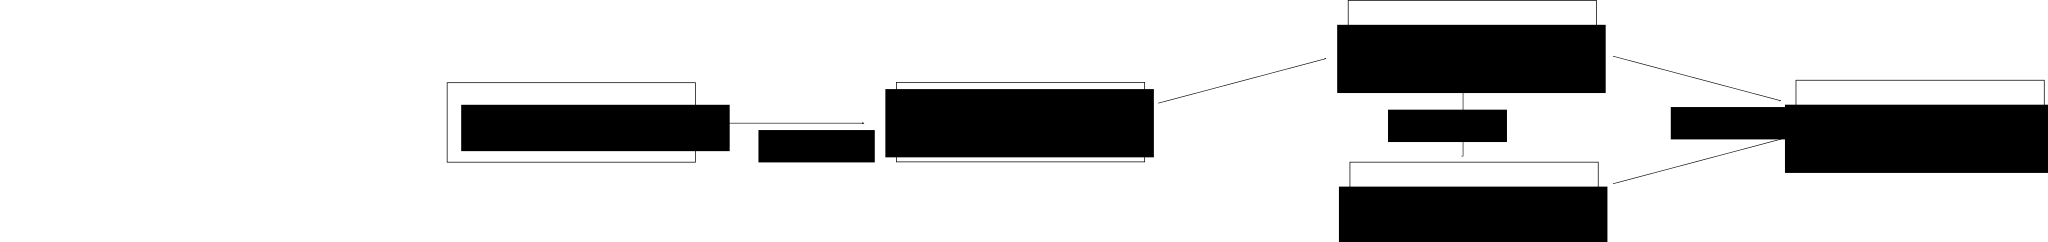
\includegraphics[width=\linewidth]{diagrams/verb-to-action-workflow.png}
        \end{center}
        \caption{The workflow for parsing an event expressed in natural lanuage into it's physical representation}
    \end{figure}

    The first step is parsing a natural language event into a predicate-argument structure relating subject and object. Each verb sense will have a definition in terms of conceptual dependencies- which CD primitive it corresponds to, and if applicable, extra attributes implied by the verb which are contingent to the primitive (e.g.~direction or polarity). This parsing process used a simple position-based system, augmented with the NLTK natural language toolkit~\cite{bird2009nltk} to assist.
    
    Primitive definitions contain information about which physical attribute it affects (e.g.~the `expel' primitive indicates the object has been removed from inside the subject, meaning an `inside\_subject' attribute is assigned to that verb), and \emph{how} that attribute changes. These attributes are used for the simulation.
    
    The verb definition is then merged with it's primitive definition (there should be no contradictory fields). This merging allows sparser verb definitions, with some information already implicit in the primitive.

    While as much of the simulation was left to unfold `naturally' as possible, to ensure the actions took place as determined by the input command some intervention was needed:

    \begin{itemize}
        \item For EXPEL events, the object was placed inside the actor, then given outwards momentum
        \item For INGEST events, the object was placed outside the actor, and given momentum towards the actor. The object of the action was made a `sensor' object in Pymunk, as Pymunk objects usually can't overlap. On entering the actor, the small object becomes attached to it via a Slide Joint, allowing the object to move freely within the radius of the absorbing object but no further
        \item For MOVE events, no specific positioning was required, but a target was queued for the radius to change as specified by the `attribute\_outcome' property
        \item For PTRANS events, a momentum was applied to the object
    \end{itemize}

    To take a more detailed example: the verbs `Expand' and `Contract' both use the MOVE primitive, as it indicates a part of the subject moving while the absolute position doesn't change. Additionally, they both have the same \emph{affected\_attribute} value of `radius'. However they clearly mean the exact opposite, so their \emph{attribute\_outcome} values differ (`increase' and `decrease' respectively).

    At this time, the MOVE attribute only applies to the radius of an object, however it would also apply to a change in shape.

    % TODO: an example with a primitive which contains some data?

    \subsection{Example: Star collapses}
    \begin{enumerate}
    \item Natural language parsing. NLTK identifies and stems the verb, in this case ``collapse''. The Subject and Object of the sentence are identified, and stored as arguments in a VerbInfo object along with the verb name. (The system also is built to handle verb sense IDs for use in larger corpora which may contain multiple definitions for the same verb- given the current system is built for a set domain, the problem of ambiguous word senses is reduced)

    \item Create CDEvent: The verb definition is looked up according to the verb name or verb sense, returning a CDDefinition object:
    
    \begin{tabular}{l l}
        \toprule
        \textbf{CDDefinition}\\
        \midrule
        affected\_attribute & EntityAttributes.radius\\
        attribute\_outcome & EntityAttributeOutcomes.decrease\\
        preceding & None\\
        primitive & Primitives.MOVE\\
        sense\_id & `collapse'\\
        \bottomrule
    \end{tabular}

    The corresponding primitive definition is looked up, returning another CDDefinition object.

    The two objects are merged into a CDEvent object, thus maintaining any keeping any data implicit in the Primitive definition. The Subject and Object items from the input sentence are set as the actor and object.
    

    \begin{tabular}{l l}
        \toprule
        \textbf{CDEvent}\\
        \midrule
        affected\_attribute & EntityAttributes.radius \\
        attribute\_outcome & EntityAttributeOutcomes.decrease \\
        event\_object & None\\
        preceding & None\\
        primitive & Primitives.MOVE \\
        sense\_id & `collapse'\\
        subject & `star'\\
        \bottomrule
    \end{tabular}

    \item Convert to ActionEvent: The CD event is converted to an array of Action events- for a compound verb definition, there will several items in the array but for many events there will only one action event. 

    Action events differ from CDEvents in that they describe exactly which physical changes need to take place for the CDEvent to be enacted, with no reference to primitives.

    \begin{tabular}{l l}
        \toprule
        \textbf{ActionEvent}\\
        \midrule
        affected\_attribute & EntityAttributes.radius\\
        attribute\_outcome & EntityAttributeOutcomes.decrease\\
        event\_object & None\\
        subject & `star'\\
        \bottomrule
    \end{tabular}

    \item Setup environment

    The Pymunk/Pygame instance is created, and the entities involved in the scenario are spawned (either a single entity or an actor and the object of that action). In the collapse example, a single Star object is created. The events which need to be simulated are `queued'- in this case, a decrease in the entity's radius. For a quantitative variable like Radius, the attribute in question is increased/decreased each frame until the target is reached. The change is halving or doubling by default.
    \end{enumerate}


    \section{Actions to Natural Language}
    \begin{figure}[h]
        \begin{center}        
            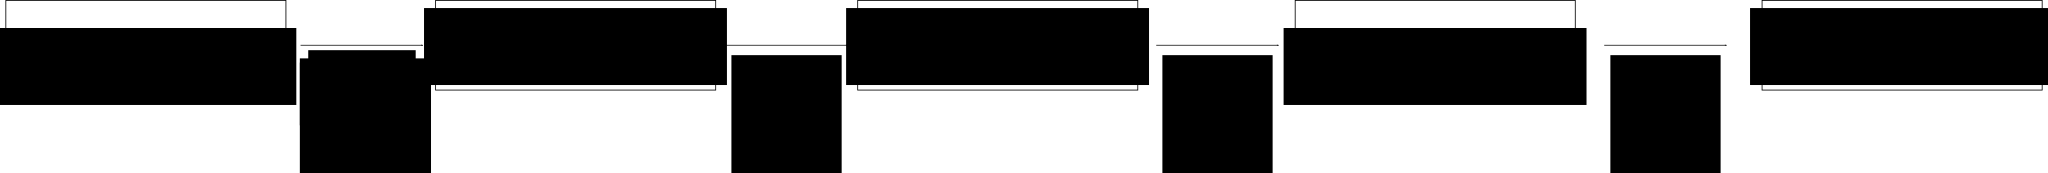
\includegraphics[width=300pt]{diagrams/action-to-verb-workflow.png}
        \end{center}
        \caption{The workflow for parsing an event expressed in natural lanuage into it's physical representation}
    \end{figure}

    Converting an event to it's Conceptual Dependencies and then into natural language uses much of the same infrastructure in reverse, with the additional aspect of an underlying physical simulation. This simulation reports notable `events' to the Manager unit, in terms of what attribute on an object was changed, and in what way.


    Primitives which contradict the information in the event are eliminated, thus restricting the candidate verbs to only those which are relevant. These are then filtered according to the remaining criteria (affected\_attribute, attribute outcome, and any selectional restrictions).

    An example of different verbs with the same primitive is `eject' and `emit'- both of these terms best correspond to the CD primitive ``EXPEL''. In a situation where a star spits out a smaller object, both of these terms will be listed as candidate verbs (and would make sense if used). However in natural language they will generally be used for different kinds of materials- `eject' will generally be used for solid structures being expelled from a larger one, whereas `emit' would generally be used for radiation or energy being expelled. This kind of constraint data can guide a system to a more appropriate choice of word.

    In this case, the system can be guided to using the more suitable verb by applying a type constraint to the object of the verb (object being used in the logical sense). Constraints in existing natural language libraries aren't generally specific enough for these purposes, so a crude list of physics-specific constraint rules was built as a proof of concept.

    \subsection{Example: Star emitting a particle}
    \begin{enumerate}
        \item A `spitting star' is created- this will have (by default) 40 particles with no initial momentum, grouped into a single CompoundEntity, which is registered with CDManager object. A single extra particle is created, with a momentum in the \(x\) direction, which is also added  as a part of the CompoundEntity.
        
        Each particle is given a random initial position in the Pymunk space, within a 200 by 200 pixel area.


\begin{lstlisting}[frame=single,caption={CDUtilities.create\_spitting\_star}]

def create_spitting_star(manager:CDManager, num_particles = None):
'Creates a star which spits out some of it\'s parts, adds it to CD manager, pymunk and pygame'
num_particles = num_particles or 40

# setup CD stuff
star = CompoundEntity()
star.name = 'Star1'

manager.objects.append(star)

for n in range(num_particles):
    x = random.randint(200, 400)
    y = random.randint(200, 400)
    ball_shape = add_ball(manager.space, x, y)
    star.parts.append(ball_shape)

ball_with_momentum = add_ball(manager.space, 300,300)
star.parts.append(ball_with_momentum)
ball_with_momentum.body.velocity = pymunk.Vec2d(80,0)


return star
    \end{lstlisting}

    \item The simulation begins, with the particles of the star attracting each other and moving towards the centre of the star. However there is enough time for the particle with initial momentum to escape the other particles, before it is enclosed.

    \item The CompoundEntity's tick method checks if any of it's component particles have strayed outside it's inclusion radius\footnote{The inclusion radius is currently defined as the mean distance of each particle from the object's centre of gravity, plus two standard deviations}.

    The tick method returns an ActionEvent object:

    \begin{tabular}{l l}
        \toprule
        \textbf{ActionEvent}\\
        \midrule
        affected\_attribute & EntityAttributes.inside\_subject\\
        attribute\_outcome & EntityAttributeOutcomes.outside\\
        event\_object & pymunk.shapes.Circle\\
        subject & CompoundEntity\\
        \bottomrule
    \end{tabular}

    \item If the system is set to print raw CD events, it will choose the appropriate primitive for the event, and print out an ASCII version of a CD diagram:
    \begin{lstlisting}
Star1 <=> EXPEL Circle
 inside_subject -> outside
    \end{lstlisting}

    \item Alternatively, if the system is set to describe events in natural language, the system looks up an appropriate verb to describe the ActionEvent. It does this by first picking the appropriate Conceptual Dependency primitive- it first eliminates any primitives which correspond to a different affected\_attribute, and then eliminates the primitive if it specifies an attribute\_outcome which doesn't match the event.

    \item Once the appropriate CD primitive has been identified, the dictionary of verbs is looped through, adding any verbs with the correct primitive and attribute\_outcome to a list of candidate verbs. One of these verbs is used to form a sentence. In this case, the verb `emit' is first on the list, so the system prints the sentence ``Star1 emits particle''

    \end{enumerate}

    \section{Physics Simulation}
    \subsection{Recognition of physical events}
    To identify discrete events in the physics simulation, objects were tracked by an object called a \textit{CDManager}. The top level script processes the effects of physical forces between the objects\footnote{At this time that is just gravity, but could be extended to include phenomena like electrostatic pressure or heat.} once per frame in the Pygame animations, then calls a `tick' method on the CDManager. \textit{CDManager.Tick} then calls the tick methods on every individual CDEntity in the simulation.


\begin{lstlisting}[frame=single,caption={CDEntity.tick method}]
def tick(self, manager):
    "Updates history of properties and returns any events"

    cog = self.get_centre_of_gravity()

    new_events = []

    # Check for particles joining or leaving
    new_events.extend(
        self._check_for_injest_or_emit(manager, cog)
    )

    # Update changing attributes
    self._update_changing_attributes()

    # Then log to histories
    cog = self.get_centre_of_gravity()
    self.cog_history.append(cog)

    history_length = len(self.cog_history)
    if history_length > 1:
        cog_delta =
            self.cog_history[history_length - 1]
            - self.cog_history[history_length - 2]
        self.cog_delta_history.append(cog_delta.get_length())

    self.radius_history.append(self.get_max_radius(cog))

    # CHECK FOR EVENTS
    new_events.extend(self._check_for_events())

    self.event_history.append(new_events)

    return new_events
\end{lstlisting}
    The CDManager object keeps track of the distances between each object in the simulation. If an entity is a `Compound' entity, it will be a cloud of small objects and it's tick method will calculate an `inclusion radius', which is determined by the standard deviation of the parts of that compound entity from it's centre of gravity. If a foreign object in the simulation has come within that inclusion radius, it will be combined into the compound entity. If one of the parts of the entity has gone outside that radius, it will be removed and the CDManager will begin tracking it as a separate CDEntity.

    The CDEntity.tick method will return a list of ActionEvent objects which have occurred. For each CD event detected, the manager will call the DetectScenarios method to try and find a matching verb to describe it:

\begin{lstlisting}[frame=single,caption={CDManager.detect\_scenarios method}]
def detect_scenarios(event:ActionEvent):
    '''Takes action events in and outputs
    candidate verbs to describe them'''
    
    selected_primitive =
        CDManager.find_primitive_for_action_event(event)            

    # Look up a verb to describe what's happened
    candidate_verbs = []

    for verb_def in verb_dictionary.values():
        if (verb_def.primitive != selected_primitive):
            continue

        if (event.affected_attribute ==
            verb_def.affected_attribute)
        and
            (event.attribute_outcome ==
            verb_def.attribute_outcome):
            candidate_verbs.append(verb_def)
    
    return candidate_verbs
\end{lstlisting}


    To avoid small fluctuations in the centre of gravity being registered as a PTRANS event, the tick method on the CDEntity only raises a PTRANS event if the centre of gravity has moved at least 5 pixels in one dimension within the past 4 ticks. The necessitates storing the centre of gravity of the object at each time slice.

    \subsection{Scripted events and queueing}
    For `scripted' events under the simulation mode, events have to be queued. The CDDefinition class has a `preceding' field, for CD events which must come before the final one in compound verbs. In the case of compound verbs such as `accrete', the first stage is set up as normal by the simulation setup script. The list of events which needs to occur is listed in the attribute\_changes property of the CDEntity- these will either take the form of a value an attribute of the entity should equal, or a CDEvent having just occurred in the entity's history. For gradual changes such as radius changes, a target value for that attribute is set, and each time the tick method is called the attribute is changed in the specified direction (increase or decrease).

    After the first `target' in attribute\_changes is met, that first cell is removed from the list so the next one can begin. This way events can take place in a set order.

    \textbf{Example: Star accretes particle}

    The `accrete' verb has two parts: the actor ingests a smaller item, then expands its radius. The setup script for the simulation will position the particle so it is moving towards the star, and set their collision handlers so the particle will attach when it enters the star, making sure it is captured. This will register a CD event which will correspond to the first target in the `attribute\_changes' list, causing the tick method to remove the first target from the list and move onto the next one. The radius will then increase by 1 pixel per tick until the target value is met.

    \begin{figure}[h]
        \begin{center}        
            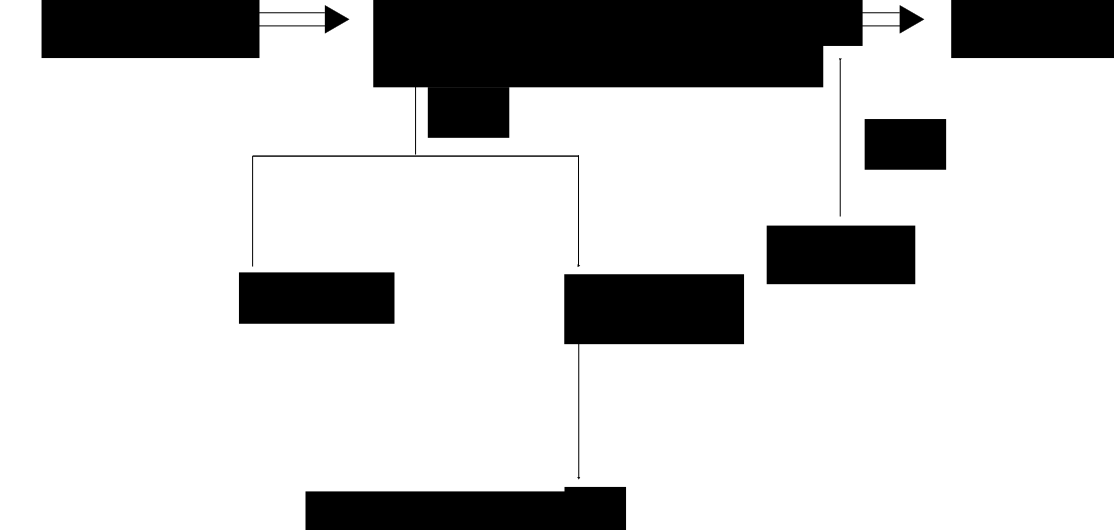
\includegraphics[width=300pt]{diagrams/accrete-cd.png}
        \end{center}
        \caption{A conceptual dependency diagram for the verb `Accrete'}
    \end{figure}


\subfile{logtalk}

    % \bibliographystyle{plain}
    % \bibliography{refs}
\end{document}